\newpage
\genHeader

% This section applies to both??
\section{Creating Instances}

\hypertarget{creatingInstance common}{}Before diving into modelling dynamic behaviour in \texttt{Part III}, let's have a brief look at how to create a concrete \emph{instance model} of your metamodel in Eclipse. In fact, we'd like to introduce you to the Leitner Box Gui! (Download THIS THING)
In the following, we use \emph{metamodel} and \emph{instance model} to differentiate between models that represent the abstract syntax and static semantics of a domain specific language (metamodel), and those that are expressed \emph{in} such a language (instance models of the metamodel).

To create an instance model, switch to your Eclipse workspace containing the generated working sets and projects from Section~\ref{sec: staticSemantics}. The Eclipse Modeling Framework (EMF) provides a generic model editor for free that allows us to create and edit an arbitrary instance of any metamodel specified with eMoflon.

Navigate to the \texttt{model} folder in your \texttt{LearningBoxLanguage} project.
Double-click the \texttt{LearningBoxLanguage.ecore} model to invoke  the \emph{Ecore model editor}.
Expand this tree to view the different classes and packages you modelled. % with EA in Sect.~\ref{sec: staticSemantics}.

To create a concrete instance of the metamodel, you must select a class which will become the root element of the new instance.
For our example, right-click the class \texttt{Box} and choose \texttt{Create Dynamic Instance\ldots} from the context-menu as depicted in Fig.~\ref{fig:context_menu}.

\begin{figure}[htbp]
	\centering
  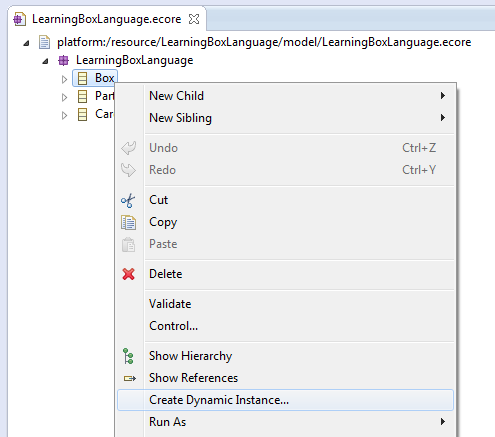
\includegraphics[width=0.5\textwidth]{eclipse_createInstance}
	\caption{Context menu of Ecore model in Eclipse}
	\label{fig:context_menu}
\end{figure}


A dialogue should pop up asking where instance model file should be persisted.
We suggest saving all your instances in a folder named \texttt{instances} that is created in every new repository project.
This is however just a convention, you are of course free to store your instances anywhere.
Last but not least, enter a name for the instance model (Fig.~\ref{fig:store_dynamic_instance}).

\begin{figure}[htbp]
	\centering
  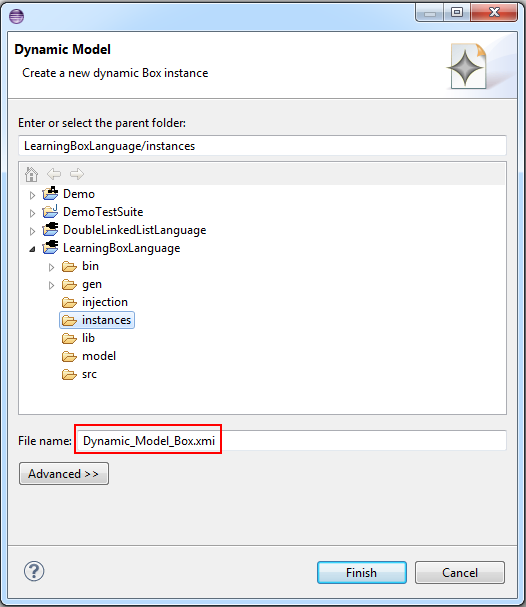
\includegraphics[width=0.4\textwidth]{eclipse_boxDynamicModel}
	\caption{Dialogue for creating a dynamic model instance}
	\label{fig:store_dynamic_instance}
\end{figure}

Now click \texttt{Finish} and the \emph{generic model editor} should be opened for your instance model.
This editor works just like the previous Ecore model editor, but it is ``generic,'' meaning it allows you to create and edit an instance of \emph{any} metamodel, not just of Ecore.
You can populate your instance model by adding new children or siblings via a right-click on an element of the instance model to invoke the context-menu depicted in Fig.~\ref{fig:create_instance}.
Note that EMF supports you by respecting your metamodel and reducing the choice of creatable elements to valid types only\footnote{This depends on the current context. Try it out!}.

\begin{figure}[htbp]
	\centering
  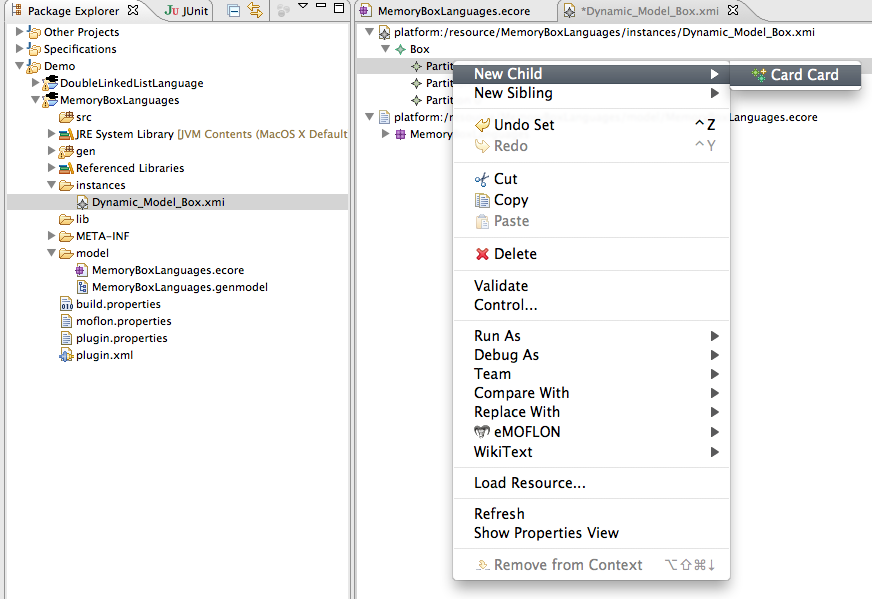
\includegraphics[width=0.8\textwidth]{adjustModel}
	\caption{Context menu for creating model elements}
	\label{fig:create_instance}
\end{figure}

You can save your model as an XMI file by pressing \texttt{Ctrl+S}.
The model can be reloaded via a simple double-click to invoke the generic model editor.

\fancyfoot[R]{ $\triangleright$ \hyperlink{conclusion}{Next} }